\section{Quasi-klassische Näherung und klassische Gase}
\subsection{Herleitung der quasi-klassischen Näherung}

Kanonisches Ensemble
\begin{align}
    \hat \rho_\text{kan} &= \frac1Z_\text{kan} \e^{-\beta \hat H} \\
    Z_\text{kan} &= \Tr \left[\e^{-\beta H}\right] \\
    \hat H &= \hat T (\hat{ \tilde p}) + W(\hat{ \tilde r}) \quad (H(\tilde p, \tilde r) \text{ klassisch analoge Hamiltonfunktion})\\
    \hat{ \tilde p} &= (\hat{\vec p}_1,\hat{\vec p}_2,...,\hat{\vec p}_N), \hat{\tilde r}=(\vec r_1,...,\vec r_N)\\ 
    \Ket{\tilde r}_s &= C (\tilde r) \hat{S}_s \Ket{r_1}^{(1)} \Ket{r_2}^{(2)} ... \Ket{r_N}^{(N)} \\
    \Braket{\hat O} &= \Tr [\rho \hat O] = \int_{\mathbb R_\text{sym}^{3N}} \dif^{3 N}\, \tilde r \, |c(\tilde r)|^2 \Braket{\tilde r|\hat S_S\, \hat \rho\, \hat O\, \hat S_S|\tilde r} \\
    &=\frac1{\cancel{N!}}\int_{\mathbb R^{3N}}\dif^{3N} \tilde r \cancel{(N!)} \Braket{\tilde r|\hat S_S\, \hat\rho \, \hat U, \hat S_S|\tilde r}\\
    \Aboxed {\hat \mathbb 1 &= \int_{\mathbb R^{3N}}\dif^{3N}\tilde p\Ket{\tilde p}\Bra{\tilde p}}\\
    \Braket{\hat O} &= \underbrace{\int_{\mathbb R ^{3N}} \dif^{3N} \tilde r \int_{\mathbb R^{3N}} \dif^3 \tilde p}_{\text{Phasenraumintegral}} \Braket{\tilde r | \tilde S_S | \tilde p}\Braket{\tilde p | \hat \rho \hat O \hat S_S | \tilde r}\\
\end{align}
\begin{align}
\intertext{Hilfsfunktion $ A_0(\vec{X})$}
    A_0(\vec x) - \Braket{\tilde p | \hat S_S | \tilde r} &\equiv \Braket{\tilde p| \hat A \hat S_S | \tilde r}
%\end{align}
%\begin{align}
\intertext{Integralkern: $ \left|\Braket{\tilde r|\hat S_S|\tilde p}\right|^2 A_0(\vec x)$}
    N=1, \hat S_S &= \hat 1\\
    \left|\Braket{\vec r_1|\hat 1| \vec p_1}\right |^2 &= \left| \frac1{2 \pi \hbar}^{\sfrac23} \e^{\frac{i}{\hbar}} \vec p_1 \vec r_1 \right|^{2?} = \frac1{(2\pi \hbar)^3} = \frac1{h^3}\\
    N > 1:  N=2\\
    &\quad\left|\Braket{\vec r_1|\Braket{\vec r_2|\frac12(1+s\hat U_{12})|p_1}|p_2}\right|^2\\
    &= \frac14 \cdot 2 \cdot \frac1{(2\pi \hbar)^6} \left| \e^{\frac{i}{\hbar} (\vec p_1 \vec r_1 + \vec p _2 \vec r_2)} + s\e^{\frac{i}{\hbar} (\vec p_1 \vec r_2 + \vec p _2 \vec r_1)} \right|^2\\
    &\quad\left[1+s\cos\left[\cancel{\frac{(\vec r_1 -\vec r_2)(\vec p_1-\vec p_2)}{\hbar}}\right])\right]\\
    \hbar &\to 0
\end{align}

\paragraph{Wiederholung}
%das haben wir schon
\begin{align}
    \Braket{\hat{O}} &= \Tr[\hat \rho \hat O]\\
    &=\int_V \dif^{3N}\tilde r \int_{\mathbb{R}^{3N}}\dif^{3N}\tilde p 
    \left|\Braket{\tilde r|\hat S_S|\tilde p}\right|^2\cdot(\rho O)_0(\vec{x})\\
    \text{Phasenraumpunkt: } \vec x &=(\underbrace{\vec r_1, \vec r_2, ...,\vec r_N}_{\tilde r}, \vec p_1,..., \vec p_N)\\
    \left|\Braket{\tilde r|S_S|\tilde p}\right|^2 &\stackrel{\hbar \to 0}{\approx}\frac{1}{(N!)^{\cancel{2}}}\cancel{N!} \frac{1}{(2\pi\hbar)^{3N}}=\frac{1}{N!h^{3N}}\\
\intertext{wir benötigen noch}
    (\rho_n O)_0(\vec x) &= \frac1{\Braket{\tilde p | \hat S_S | \tilde r}} \Braket{\tilde p | \hat \rho \hat O \hat S_S | \tilde r}
\end{align}
%\begin{enumerate}[(1)]
%    \item 
        \begin{align}
            \hat{O} = \hat{1} \Rightarrow (\hat{\rho}_k)(\vec{x}) &= ... \\
            \Braket{\tilde p|\hat \rho\hat S_S|\tilde r} & =\frac{1}{Z}\Braket{\tilde p|\e^{-\beta (\hat T+\hat V)}S_S|\tilde r}\\
            \e^{-\beta (\hat T+\hat V)} &\approx \underarrow{\e^{-\beta \hat T}}{\text{nicht exakt da, }[\hat V, \hat T] \neq 0} \e^{-\beta \hat V} + \mathcal O(\beta\hbar) \\
            \hat T&=\sum_{j=1}^{N}\frac{1}{2}\vec{\hat p_j}^2\\
            [\hat{V},\vec{p}\vec{p}] &= [\hat{V},\underarrow{\vec{p}}{\frac{\hbar}{i}\vec{\nabla}}]\vec{p} + \vec{p}[\hat{V},\vec{p}] = -\frac{\hbar}{i}(\nabla V)\vec{p} - \frac{\hbar}{i} \vec{p}(\nabla V)\\ 
            &= \hbar^2 (\increment V) - \frac{2 \hbar}{i} (\vec \nabla) \vec p = \mathcal O(\hbar)\\
            \Braket{\tilde p|\e^{-\beta (T+V)}\hat S_S|\tilde r} &\approx \e ^ {-\beta T(\tilde p)} \e^{- \beta V(\tilde r)} \Braket{\tilde p | \hat S_S | \tilde r} + \mathcal O (\beta \hbar)\\
            \beta \to 0 \ &\hat= \ \text{Hochtemperaturnäherung}\\
            (\rho)(\vec x) &= \underarrow{\rho}{\text{klassische Dichte im Phasenraum}}(\vec x)
            =\frac{1}{Z}\symup{e}^{-\beta H(\vec x)}, \quad H: \text{klassische Hamiltonfunktion} \\
            (\hat \rho \hat O)_0(\vec{x}) &\longrightarrow \rho(\vec x)O(\vec{x})\\
        \intertext{für $\hbar \beta \to 0$: Hochtemperaturlimes}
            \Braket{\hat O}&=\frac{1}{N!}\int \underbrace{\frac{\dif^{6N}\vec x}{(2\pi\hbar)^{3N}}}_\text{dimensionslos}\frac{1}{Z_\text{quasikl.}}\symup{e}^{-\beta H(\vec{x})}\mathcal O(\vec x)\\
            \Rightarrow Z_\text{quasikl.} &= \frac1{N!} \int \dif^{3N} \tilde r \int \frac{\dif^{3 N} \tilde p}{h^{3 N}} \e^{-\beta H(\vec x)}\\
        \intertext{Impulsintegration}
            \int_{-\infty}^{\infty} \symup{d}p_{j\alpha} \symup{e}^{-\frac{beta}{2m}p_{j\alpha}^2} &= \sqrt{2 m k_\text{B} T \pi} \\
            \alpha=1,2,3 \quad \int_{-\infty}^{\infty}\dif x\symup{e}^{-x^2} &=\sqrt{\pi} \ ; \ \dif X= \frac{1}{\sqrt{2\pi k_\text{B} T}}\dif p\\            
        \intertext{Thermische de-Broglie-Wellenlänge}
            \Lambda_T &= \frac{2\pi}{\sqrt{2 m k_\text{B} T \pi}}\\
% Bild 13 das ist wieder ne richtig gute Zeichnung NICHT
          \Aboxed{  Z_\text{quasikl.} &= \frac1{N!} \int \frac{\dif^{3N} \tilde r}{(\Lambda_T)^{3N}} \e^{-\beta V(\tilde r)}}\\
        \end{align}
%\end{enumerate}

\subsubsection{Gleichverteilungssatz}

Klassische Observable
\begin{align}
    O &= p_{j\alpha} \pdif{H}{p_{j\alpha}}\\
\intertext{wir verwenden:}
    \symup{e}^{-\beta H(\vec x)} &=- \frac1{\beta} \pdif{}{p_{j\alpha}} \e^{-\beta H}\\
\intertext{partielle Integration:}
    \int_\infty^\infty\dif p_{j\alpha}\underbrace{\pdif{H}{p_{i\alpha}}\symup{e}^{\beta H(\vec x)}}_{-\frac{1}{\beta}\pdif{}{p_{j\alpha}}\symup{e}^{-\beta H}} 
    &= -\cancel{\frac1\beta p_{j \alpha }\e^{-\beta H}} \biggr\rvert_{-\infty}^\infty + \frac1\beta \int_{-\infty}^\infty \dif p_{j \alpha} \e^{-\beta H(\vec x)}\\
    \Rightarrow \Aboxed{\Braket{p_{j\alpha}\pdif{H}{p_{j\alpha}}} &= k_\text{B} T}
\end{align}
\paragraph{Anwendung}
\begin{align}
    H&=\sum_{j=1}^N \frac{p_j^2}{2m}+V(\tilde r)\\
    \Braket{\frac{p_j^2}{2m}} &=\frac{1}{2}\sum_\alpha \Braket{p_{j\alpha}\pdif{H}{p_{ja}}}=\frac{3}{2}k_\text{B} T\\
    \Rightarrow \frac12 k_\text{B} T &\quad \text{pro Freiheitsgrad}\\
    \text{ideales Gas:  } V(\tilde r) &= 0\\
    U&=\frac{3}{2}k_\text{B} T N\\
\intertext{Sp. Wärme}
    C_V=\pdif{\Braket{H}}{T}[V]=\frac{3}{2}N k_\text{B}
\end{align}

\subsubsection{Entropie}
Ideales Gas: $V(\tilde r) = 0$
\begin{align}
    Z_\text{quasikl.} &= \frac{1}{N!} \left( \frac{V}{\lambda_T^3} \right)^N
\intertext{Stirling Formel} 
    N! &\stackrel{N\to\infty}{\approx} \sqrt{2 \hbar N} \left(\frac Ne \right)^N \propto N^N\\
    \ln\left(Z_\text{quasikl.}\right) &= \ln\left( \frac1{N!} \left( \frac{V}{\lambda_T^3} \right)^N \right) \\
    &\approx \ln\left(\frac{1}{\sqrt{2\pi N}}\left(\frac{V\e}{N\lambda_T^3}\right)^N\right)
    &= N \ln \bigg( \underarrow{\frac{V}{N}}{\parbox{3cm}{$N \to \infty \Rightarrow \frac VN = \frac1n$ \\ inverse Dichte}} \frac{e}{\lambda_T^3} \bigg) - \frac1{2} \ln\underarrow{\cancel{(2 \pi N)}}{\parbox{2.5cm}{subextensiv \\$ \frac1N \ln N \stackrel{N\to \infty}{\to} 0$}} \\
    \ln Z&: \,\,\text{Extensiv} 
\end{align}
Freie Energie 
\begin{align}
    F(T,V)=-\frac{1}{\beta}\ln(Z_\text{quasikl.})=-N k_\text{B} T \ln\left(\frac{V}{N}\frac{\e}{\lambda_T^3}\right)\\
    \intertext{Zustandsgleichung}
    \label{eqn:p}
    p = -\pdif{F}{V} = -\left(-N k_\text{B} T \frac{1}{V} \right) \quad \Rightarrow \Aboxed{p V = N k_\text{B} T}
\end{align}
\paragraph{Entropie}
\begin{align}
    S&=-\pdif{F}{T}=N k_\text{B} \ln \left( \frac{V}{N} \frac{\e}{\lambda_T^3} \right)-k_\text{B} T N\frac{1}{\lambda_T^3}\left(\pdif{\lambda_T^3}{T}\right)\\
    \Lambda_T^3 &= C T^{-\frac32}\\
    \pdif{\Lambda_T^3}{T} &=- \frac32 C T^{-\frac32} \frac1T = -\frac32 \Lambda_T^3 \frac1T\\
    S &= N k_\text{B} \left[\ln\left(\frac{V}{N}\frac{\e}{\lambda_T^3}\right)+\frac32\right]
\end{align}
\paragraph{Gesamtenergie}
\begin{align}
    U &= F + TS = \frac32 N k_\text{B} T = U(S, V)
\end{align}
\paragraph{Enthalpie}
\begin{align}
\intertext{mit \eqref{eqn:p}}
    H(S,N,p) &= U + pV = \frac32 N k_\text{B} T +  N k_\text{B} T= \frac52 k_\text{B} T N\\
    C_p &= \pdif{H(S,p)}{T}=\frac52 k_\text{B} N 
\end{align}

\paragraph{Wiederholung}

\begin{align}
    C_v &= \frac32 N k_\text{B}, \quad V = \text{const.} \\
    C_p &= \frac52 N k_\text{B}, \quad p = \text{const.} 
\intertext{Wärmeausdehnungskoeffizient $\alpha$}
    \alpha &= \frac{1}{V} \pdif{V}{T}[p,N]=\frac1V \pdif{}{T} \left(\frac{N k_\text{B} T}{p}\right)= \frac{N k_\text{B}}{p V}\frac{T}{T}= \frac1T
\intertext{Zustandsgleichung}
    pV &= N k_\text{B} T
\intertext{Isotherme Kompressibilität $\varkappa_T$}
    \varkappa_T &= -\frac{1}{V}\pdif{V}{p} = -\frac1V\pdif{}{p}\left(\frac{N k_\text{B} T}{p}\right)
    =\underbrace{\frac{N k_\text{B} T}{Vp}}_{=1} \frac1p = \frac1p\\
    \frac{C_V}{C_p} &=\frac{\varkappa_S}{\varkappa_T}\Rightarrow \varkappa_S=\varkappa_T \frac{C_V}{C_p}=\frac1p \frac{\frac{3}{\cancel{2}}\cancel{N k_\text{B}}}{\frac{5}{\cancel{2}}\cancel{N k_\text{B}}} = \frac35 \frac1p\\
    \Lambda_T&=\frac{2\pi}{\sqrt{2\pi m k_\text{B} T}}
\intertext{Klassisch: $l_0 \gg \lambda_T$}    
\intertext{QM: $l_0 \ll \lambda_T$}
\intertext{$l_0$ natürlichen Längenskala des Problems}
    \text{Gas: } l_0&=\sqrt[3]{\frac VN}
\intertext{Elektron im Festkörper?}
    l_0 &= \SI{1e-10}{\meter} \\
\end{align}

Bei welcher Temperatur geschieht der Übergang QM \rightarrow Kl?
\begin{align}
    \lambda_T^2&=l_0^2\\
    \frac{(2\pi \hbar)^2}{2\pi m k_\text{B} }\frac{1}{l_0^2} &=T=\frac{2\pi (\hbar c)^2}{\underbrace{m c^2}_{E_e}k_\text{B}}\frac{1}{l_0} = \frac{2\pi (\SI{197}{\mega\electronvolt\femto\meter})^2}{\SI{0.5}{\mega\electronvolt}(\SI{1e5}{\femto\meter})^2} \frac{1}{k_\text{B}}
    =\frac{\SI{47}{\electronvolt}}{k_\text{B}}=\SI{540000}{\kelvin}
\end{align}
$\Rightarrow$ Elektronen müssen quantenmechanisch behandelt werden!

\subsection{Bohr--van-Leeuwen--Theorem}
\begin{align}
    \text{Klassisch:}\quad H(\underarrow{\vec X}{\text{Phasenraumpunkt}},\vec A(\vec r_i)) &= \frac1{2n} \sum_{i=1}^N \left(\vec p - \frac ec \vec A (\vec r_i)\right)^2 + V (\tilde r) \\
    Z_\text{quasikl.} (\vec A) &= \frac1{N!}\int \frac{\dif^{3N}\tilde{r}}{(2\pi \hbar)^{3N}} \e^{-\beta V(\tilde{r})} 
    \int \dif^{3N}\tilde p \e^{-\beta\frac1{2n} \sum_{i} \underbrace{\left(\vec p_i - \frac ec \vec A\right)^2}_{(\vec p_i')^2}}\\ 
    &= Z_\text{quasikl.} (\vec A = 0)\\
    \vec p_i' &= \vec p_i - \frac ec \vec A \\
    \vec M_\text{kl.} &= -\pdif{F(T,V,B)}{\vec B} = 0
\intertext{$\Rightarrow$ Magnetismus ist ein Quanten-Phänomen}
\end{align}

\subsection{Cluster- und Virialentwicklung}
\begin{align}
    Z_\text{quasikl.} &= \frac{1}{N!}\int_V \frac{\dif^{3N}\tilde r}{(\Lambda_T^3)^N} \e^{-\beta V(\tilde r)} 
\intertext{Zweiteilchen-Wechselwirkung}
    V(\tilde r) &= \sum_{j<l} v(\vec r_j - \vec r_l) = \sum_{j<l} v_{jl}, \qquad \frac{N(N-1)}{2}\ \text{Terme}
\intertext{Abweichung von idealen Gasen}
    Q(T,V,N) &\equiv \underbrace{\frac{N! \Lambda_T^{3N}}{V^N}}_{=\frac1{Z_\text{quasikl.}} \ \text{ideales Gas}} Z_\text{quasikl.}
\intertext{Referenz $Q=1$, für $\beta v(\tilde r) = 0$}
\intertext{Hilfsgröße}
    f_{jl}&= \left(\e^{-\beta v_{jl})}-1\right) \ge -1
\end{align}
\begin{figure}[H]
  \centering
  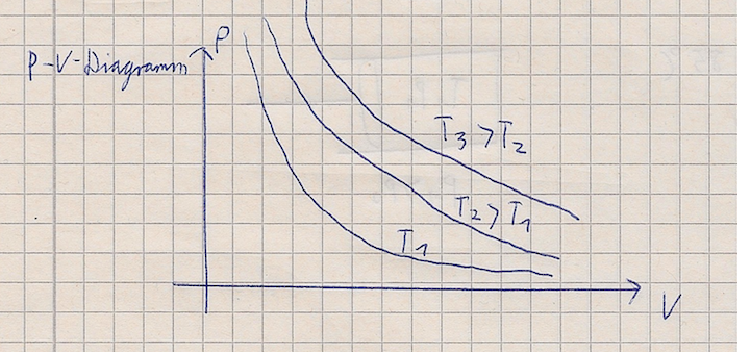
\includegraphics[width = \textwidth]{Zeichnungen/14.pdf}
  \caption{p-V-Diagramm bei verschiedenen Temperaturen.}
  %\label{fig:Bild14}
\end{figure}
\begin{align}
    \text{Für} |\beta v_{jl}| \ll: f_{jl} &\hat= 1-\beta v_{jl} -1 + \mathcal O ((\beta v)^2)\approx -\beta v_{jl}\\
    \Rightarrow |f_{jl}|&\approx|\beta v_{jl}| 
\intertext{Gewichte:}
    \e^{-\beta V(\tilde{r})} &= \prod_{j<l}(1+f_{jl}) = \left(\prod_{j<l} \e^{-\beta v_{jl}}\right) \\
    Q(T,V,N) &= \int_V \frac{\dif^{3N} \tilde r}{V^N} \underbrace{\prod_{j<l} (1+ f_{jl})}_{2^{\frac{N(N-1)}{2}} \text{Terme}} \\
    &= \int_V \frac{\dif^3N \tilde r}{V^N} \left[\underbrace{1}_{(a)} + \underbrace{\sum_{j<l} f_{jl}}_{(b)} + \sum_{j<l} \sum_{\substack{m<n \\ (j,l) \neq (m, n)}} f_{jl} f_{mn} + ... \right] 
\end{align}
\paragraph{Terme graphisch darstellen:}
\begin{enumerate}[i)]
    \item Jedes Teilchen hat einen Index \circled{$i$}
    \item $f_{jl}$: Verbindungslinien zwischen $j$ und $l$: \circled{$j$} $\underarrow{\longleftrightarrow}{f_{jl}}$ \circled{$l$} 
    \item Das Potential hängt nur vom Relativabstand ab, ne?
        \begin{align}
            \int \dif^3 (\vec r_j-\vec r_i) f(\increment \vec r)
        \end{align}
\end{enumerate}

Beispiel $N=3: \# = 2 ^ \frac{3\cdot2}{2} = 2^3 = 8$:

%\begin{enumerate}[(a)]
%    \item  $\circled{1} \qquad \circled{2} \qquad \circled{3}$
%    \item $\circled{1} \rule[3pt]{2em}{1.2pt} \circled{2} \qquad \circled{3} \qquad \qquad \circled{1} \qquad \circled{2}\rule[3pt]{2em}{1.2pt}\circled{3} \qquad \qquad \underbracket{\circled{1} \qquad \circled{2} \qquad \circled{3}}$
%    \item $\circled{1}\rule[3pt]{2em}{1.2pt}\circled{2}\rule[3pt]{2em}{1.2pt}\circled{3} \qquad \qquad \underbracket{\circled{1}\rule[3pt]{2em}{1.2pt}\circled{2} \qquad \circled{3}} \qquad \qquad \underbracket{\circled{1} \qquad \circled{2}\rule[3pt]{2em}{1.2pt}\circled{3}} $
%    \item  $\underbracket{\circled{1}\rule[3pt]{2em}{1.2pt}\circled{2}\rule[3pt]{2em}{1.2pt}\circled{3}} $
%\end{enumerate}

\begin{enumerate}[(a)]
    \item  $\cluster[1] \quad \cluster[2] \quad \cluster[3]$
    \item $\cluster[1][2] \quad \cluster[3] \qquad \cluster[1] \quad \cluster[2][3] \qquad \underbracket{\cluster[1] \quad \cluster[2] \quad \cluster[3]}$
    \item $\cluster[1][2][3] \qquad \underbracket{\cluster[1][2] \quad \cluster[3]} \qquad \underbracket{\cluster[1] \quad \cluster[2][3]}$
    \item $\clustertri{1}{2}{3}$
\end{enumerate}

\begin{align}
    \left[\cluster\right] &= 1 \qquad \left[ \cluster[1][2][3] \right] = \left[\cluster\right]^3 = 1^3 = 1 \\
    \left[\cluster[][]\quad\cluster \right] &= \underarrow{\left[\cluster[][]\right]} {\text{zusammenhängender Cluster}} \left[ \cluster \right]\\
    \left[\cluster[][]\right]&=\int\int_V \frac{\dif^3 r_1 \dif^3 r_2}{V^2} = \frac 1V \int \dif^3 r' f(\vec r') \\
    \left[\cluster[][][]\right] &= \int \int \frac{\dif r_{12} \dif r_{23}}{V^2} f_{12} f_{23} = \left[\cluster[][]\right]^2\\
    \left[\clustertri{}{}{}\right]&=\int\int\frac{\dif r_{12} \dif r_{23}}{V^3} f_{12}f_{23}f_{31}\\
    Q(T,V,N=3)&=\left[\cluster\right]^3+3\left[\cluster\right]\left[\cluster[][]\right]+3\left[\cluster[][][]\right]+\left[\clustertri{}{}{}\right]=\left[\cluster[][]\right]^2
\end{align}

%HIER FEHLT WAS SIEHE FOTO

\begin{align}
	Q &= Z_\text{quasikl.} \frac{N! \Lambda^{3N}_T}{V^N}\\
	N &= 3\\
    Q(T,V,N=3)=&\underarrow{\left[\cluster\right]}{C_1}^3\\
    &+ 3\left[\cluster[] \quad \underbrace{\cluster[][]}_{C_2}\right] \leftarrow\text{Graph}\\ 
    &+3\left[\cluster[][][]\right]\leftarrow C_3\\
    &+\left[\clustertri{}{}{}\right]\leftarrow C_4
\end{align}

\paragraph{Graph:} $N$ Punkte (Kugeln) \\
Zerfällt in Cluster mit $n_j$ Punkten  \\
Cluster tritt $m_j$ mal im Graphen auf 
\begin{align}
	\Rightarrow N &= \sum^\infty_{j=1} m_j n_j \quad m_j = 0, 1, …\\
	\frac1{V^{n_j - 1}} &= \frac1{N^{n_j -1} V^{n_j -1}}\\
	\theta &= \frac VN \quad \text{mittleres Volumen pro Teilchen (intensiv)}
\intertext{Integration: \quad  $v(|\vec r |)$  wirkt auf der Skala $r_0$ }
    I &\propto \left( \frac{{r_0}^3}{v}\right) \quad \text{intensiv}
\end{align}

\paragraph{Frage:} Vielfachheit eines Graphen gleicher Topologie: L?
\begin{itemize}
    \item $N!$ Möglichkeiten die Kugeln zu nummerieren
    \item Nicht alle führen zu verschiedenen Beiträgen
\end{itemize}

\begin{enumerate}
    \item mehrere Kopien $C_j$ im gleichen Graphen:
        \begin{align}
            \text{d.h.: } &m_j >1\\
            \left[\cluster[1][1]\right]\left[\cluster[3][4]\right] &= \left[\cluster[3][4]\right]\left[\cluster[1][2]\right] \\
            m_j! &\quad \text{Möglichkeiten}\\
        \end{align}
    \item Cluster $C_j$ kann auf $s_j$ verschiedene Arten in der Ebene gezeichnet werden.
        \begin{align}
            \left[\clustertri{1}{2}{3}\right] = \left[\clustertri{3}{1}{2}\right] = \left[\clustertri{1}{3}{2}\right] = \left[\clustertri{2}{3}{1}\right] = …
        \end{align}

        \begin{align}
            S_4 &= 6\\
            \left[\cluster[1][2]\right] &= \left[\cluster[2][1]\right] \Rightarrow  S_2=2\\
            \left[\cluster[1][2][3]\right] &= \left[\cluster[3][2][1]\right] \quad S_3 =2\\
            \Aboxed{L &= \frac{N!}{\prod_{j = 1}^{\infty}} (m_\text{j}! S_\text{j}^{m_\text{j}})}\\
        \intertext{Beispiel}
            \sigma_1 =\left[\cluster\right]^3:     \qquad L&=\frac{3}{1^3 3!}= 1 \checkmark\\ 
            \sigma_2 = \left[\cluster\right]\left[\cluster[][]\right]: \qquad L&= \frac{3!}{1^1 \cdot 1^1 \cdot 1! \cdot 2^1} = \frac{3!}{2} = 3 \\
            \sigma_3 = \left[\cluster[][][]\right]: \qquad L&=\frac{3!}{1!2}=3 \checkmark \\
            \sigma_4 = \left[\clustertri{}{}{}\right]: L&=\frac{3!}{6 \cdot 1!} =1 \checkmark
        \end{align}
\end{enumerate}

\begin{align}
    Q(T,V,N) &\underarrow{=}{N=\sum_{j=1}^{\infty} m_j n_j} \sum_{\{m_j\}} N! \prod_{j=1}^\infty \frac1{m_j!} \frac{C_j}{S_j}^{m_S} \\
    Z_\text{quasikl.}&=\sum_{\{k_j\}} \prod_{j=1}^{\infty} \frac{1}{m_j!}\left[\left(\frac{V}{\Lambda_T^3}\right)^{n_j}\frac{C_j}{S_j}\right]^{m_j} \\
    \left(\frac{V}{\lambda_T^3}\right)^{n_j} C_j &= \frac{V}{\lambda_T^3} C_j'\\
    C_j: \quad \int\frac{\dif^3r}{V} &\longrightarrow \int \frac{\dif^3r}{\Lambda_T^3}  \quad \text{in } C_j' 
\intertext{kanonisch $\rightarrow$ großkanonisch}
    \underarrow{Z_\text{quasikl., gk}}{Z = \e^{\beta \mu}}(T,V, \mu) &= \sum_{N=1}^{\infty} z^N Z_\text{quasikl.}(T,V,\mu) \\
    &=\sum_{m_j, \text{frei}} \prod_{j=1}^{\infty} \frac{1}{m_j!} \biggl[ z^{n_j} \frac{V}{\lambda_T^3} \frac{c_j'}{s_j} \biggr] ^{m_j} \\
    Z_\text{quasikl.}^\text{gk.}(T,V,m)&=\prod_{j=1}^{\infty}\left[\sum_{m_j}^{\infty} \frac{1}{m_j!}\left[z^{n_j}\frac{v}{\lambda_T^3}\frac{c_j'}{s_j}\right]^{m_j}\right]\\
    &= \e^{\frac{V}{\lambda_T^3} \sum_{j=1}^\infty \left[z^{n_j} \frac{c_j'}{s_j}\right]}\\
\end{align}

Summe über alle Clusterbeiträge exponenzieren!
\paragraph{Linked-Cluster-Theorem}
großkanonisches Potential:
\begin{align}
    \Phi(T,V,\mu)=-\frac{1}{\beta}\ln (Z_\text{quasikl.}^\text{gk})=-\frac{V}{\lambda_T^3}\left( \sum_{j=1}^{\infty}\left(z^{n_j}\frac{c_j'}{S_j}\right)\right)   
\end{align}

\paragraph{Zustandsgleichung}
\begin{align}
    p&=-\pdif{\Phi}{V}\\
    \frac{p}{k_\text{B} T} &= \frac{1}{\lambda_T^3} \sum_{j=1}^{\infty} [z^{n_j}\frac{C_j'}{S_j}]\\
\intertext{Alle Cluster mit fester Teilchenzahl $l \,\,\, (n_j = l)$}
    b_l&=\sum_{j=1}^\infty \frac{C_j'}{S_j}\\
    \Aboxed{\frac{p}{k_\text{B} T} &= \frac1{\lambda_T^3} \sum_{l=1}^{\infty} z^l b_l}
\end{align}
\begin{align}
    b_1 &= c_1 = 1\\
    b_2 &= \frac{C_2}{2} = \frac{1}{2} \int \frac{\dif^3 r}{\lambda_T^3} f(\vec r)
\end{align}
\paragraph{Teilchenzahl}
\begin{align}
    N &= -\pdif{\Phi}{\mu} = \frac{V}{\lambda_T^3} \sum_{l=1}^{\infty} l z^l b_l\\
    \frac{1}{v} &= \frac{1}{\lambda_T^3} \sum_{l=1}^\infty l z^l  b_l\\
\intertext{Virialentwicklung}
    \frac{pV}{k_\text{B}T} &= \sum_{l=1}^{\infty} a_l(T) \left(\frac{\lambda_T^3}{V} \right)^{l-1} \qquad \text{Korrektur zum idealen Gas}\\
\intertext{Unbekannte Virialkoeffizienten: $a_l(T)$}  
\intertext{linke Seite}
    \frac{pV}{k_\text{B} T} &= \frac{\cancel{\frac{1}{\lambda_T^3}} \sum_{l=1}^{\infty} z^l b_l}{\cancel{\frac{1}{\lambda_T^3}} l z^l b_l} \\
\intertext{rechte Seite}
    &= \sum_{l=1}^\infty a_l(T) \left(\sum_{n=1}^\infty n z^n b_n\right)^{l-1}\\
    \sum_{l=1}^\infty z^l b_l &= \left( \sum_{l=1}^\infty l z^l b_l\right)\left(\sum_{l=1}^\infty a_l(T) \left(\sum_{n=1}^\infty n z^n b_n\right)^{l-1}\right)
\end{align}
Für beliebige $Z$  muss die Gleichung gelten:
\begin{align}
    \Rightarrow a_1&=1\\
    a_2&=-b_2=\frac{1}{2}\int \frac{\dif^3 r}{\lambda_T^3} f(r)\\
    a_3 &= 4 b_2^2 - 2 b_3
\end{align}
\paragraph{Virialentwicklung (Wdh.)}
\begin{align}
    \frac{pV}{k_\text{B} T} &= \sum_{l=1}^{\infty} a_l(T) \left(\frac{\lambda_T^3}{V} \right)^{l-1} \left(\frac{r_0^3}{r_0^3}\right)^{l-1} \\
    a_1 &= 1\\
    a_2 &= -b_2 = -\frac12\int \frac{\dif^3 r}{\lambda_T^3} f(\vec r) \quad \text{mit} \quad f(\vec r) = \e^{-\beta U(\vec r)} -1 \\
    a_3 &= 4b_2^2 -2b_3\\
    \frac{pV}{k_\text{B} T} &= \sum_{l-1}^{\infty} a_l'(T) \left( \frac{r_0^3}{V} \right)^{l-1} & \\
    a_l'(T) &= a_l(T) \left(\frac{\lambda_T^3}{r_0^3} \right)^{l-1} \\ 
\end{align}

\subsubsection{Die van-der-Waals-Gleichung}
\begin{align}
    f(|\vec r|) &= 
    \begin{cases}
    -1 &\ |r| \leq 2 r_0\\
    \approx - \beta U(|\vec r|) &\text{ für } |\vec r| > 2 r_0
    \end{cases}\\
    a_2' &= -\frac12 \int \frac{\dif^3 r}{r_0^3} f(\vec r) = \frac12 \int_{|r| < 2r_0} \frac{\dif^3}{r_0^3} + \frac{\beta}{2} \int_{|r| \geq 2r_0} \frac{\dif3}{r_0^3} U(\vec r) = \underarrow{B}{\text{Hardcore-Abstoßung\hspace{2cm}}} - \underarrow{\frac A{k_\text{B} T}}{\text{\hspace{1cm}van-der-Waals-Anziehung}} \\ 
    B &= \frac1{2 r_0^3} \frac{4\pi}{3} (2 r_0)^3 = \frac{16}{3} \pi\\
    A &= - \frac12 \int_{2 r_0 < |r|} \frac{\dif^3 r}{r_0^3} = - 16 \pi \int_1^\infty \dif x x^2 U(2 r_0 x) \geq 0\\
    \frac{p V}{k_\text{B} T}&=1+\underarrow{\left(B-\frac{A}{k_\text{B} T}\right)}{a_2'(T)} \left(\frac{r_0}{V}\right)=1+B\frac{r_0^3}{V} - \frac{A r_0^3}{k_\text{B} T V}\\ &
    \approx \frac{1}{1-B \frac{r_0^3}{V}} - \frac{A r_0^3}{k_\text{B} T V}  \quad \biggr| \left(1-B\frac{r_0^3}{V}\right) \\
    pV\left(1- \frac{B r_0^3}{V}\right) &= k_\text{B} T - \frac{A r_0}{V} \left(1- \frac{B r_0^3}{V}\right)
\intertext{es folgt die van-der-Waals-Gleichung: }
    \Rightarrow k_\text{B} &\approx \underbrace{\left(p + \frac a{V^2}\right)}_\text{eff. Druck}\underbrace{(V-b)}_{\text{eff. Volumen}} \quad \intertext{mit} \quad a &= A r_0^3, \ \underarrow{b = B r_0^3}{\text{\enquote{Molekülvolumen}}}
\end{align}
\paragraph{Zustandsgleichung des idealen Gases}
\begin{align}
    pV &= k_\text{B} T \Rightarrow p=\frac{k_\text{B} T}{V} \\ 
    \Rightarrow \underarrow{\left(\pdif{p}{V}\right)_T}{\text{Steigung der Isothermen}} &= - \frac{k_\text{B} T}{V^2} < 0 \\
%Bild(14)
    \text{van-der-Waals-Gl.:} \quad \frac{k_\text{B}T V^2}{p} &= \left(V^2 + \frac a{p} \right)(V-b) = V^3 + \frac{aV}{p} - bV^2 - \frac{ab}{p} \\
    V^3 - \left(b + \frac{k_\text{B} T}{p}\right) V^2 + \frac{a}{p} V - \frac{a b}{p} &= 0 
\end{align}
Kubische Gleichung: 1 Lösung oder 3 Lösungen

\begin{figure}[H]
  \centering
  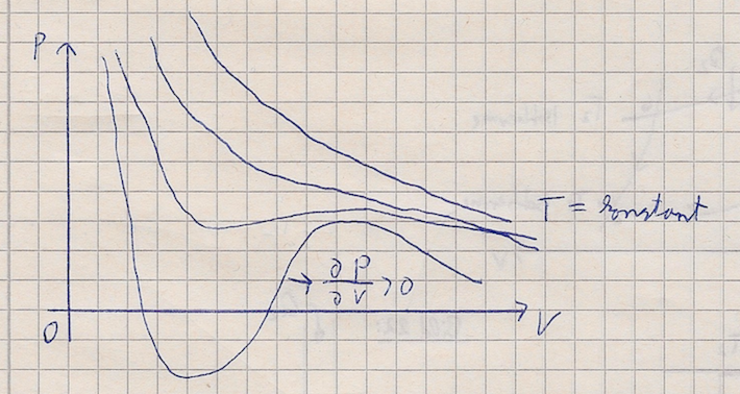
\includegraphics[width = \textwidth]{Zeichnungen/15.pdf}
  \caption{p-V-Diagramm mit positiver Steigung.}
  %\label{fig:Bild}
\end{figure}

\paragraph{Fragen:}
\begin{enumerate}
    \item  Wann 1 Lösung, wann 3 Lösungen?
    \item  Wenn 3 Lösungen: Welche ist die Richtige?    
\end{enumerate}

\paragraph{Kritischer Punkt: $V = V_C$} 
\begin{align}
    (V-V_C)^3 = 0 \\
     V^3 - 3 V^2 V_C + 3 V V_C^2 - V_C^3 = 0\\
\intertext{Koeffizientenvergleich:}
    V_C^3=\frac{ab}{p_C}  \quad ;\quad 3V_C^2&=\frac{a}{p_C}\\
    3 V_C &= (b+\frac{k_\text{B} T_C}{p_C}) \\
    \text{kritisches Volumen: } V_C &= 3 b\\
    \text{kritischer Druck: } p_C &= \frac{a}{3V_C^2} = \frac{a}{27b^2} \\
    k_\text{B} T_C &= \frac{8 a}{27 b}
\end{align}

\paragraph{Dimensionslose Einheiten:}
\begin{align}
    \bar{p} &= \frac{p}{p_C} \\
    \bar{V} &= \frac{V}{V_C} \\
    \bar{T} &= \frac{k_\text{B}}{k_\text{B}} \frac{T}{T_C}\\
\intertext{Einsetzen in die van-der-Waals-Gleichung führt auf: }
    \Rightarrow \Aboxed{\frac83 \bar{T} &= \left( \bar{p} + \frac3{\bar{V}^2} \right)\left(\bar{V} -\frac1{3}\right)} \quad \text{Universalität} \\
    \bar{p}&=\frac{8 \bar T }{3 \bar V-1 }-\frac{3}{{\bar V}^2 }\\
    \pdif{\bar{p}}{\bar{V}} &= -\frac{8\bar{T}}{3\left(\bar{V}-\frac1{3}\right)} = -\frac{6}{\bar{V}^3} \left[ \frac{4 \bar{T}  \bar{V}}{\left(3-\frac1{V}\right)^2} - 1 \right]
    \pdif{\bar p}{\bar V} \quad \Rightarrow \quad \text{kritischer Punkt} \\
\end{align}

\begin{figure}[H]
  \centering
  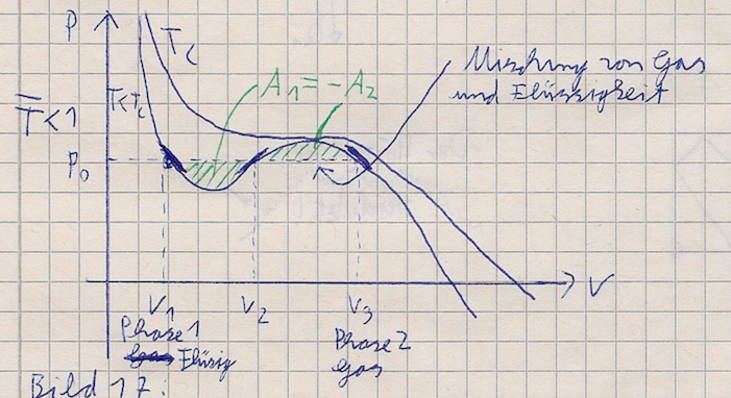
\includegraphics[width = \textwidth]{Zeichnungen/16.pdf}
  \caption{p-V-Diagramm mit Phasenübergängen.}
  %\label{fig:Bild}
\end{figure}
\paragraph{Freie Energie}
\begin{align}
   T \quad &\text{Fest}\\
   F(T,V) &= F(T,V_1) - \int_{V_1}^{V} \dif V p(V)
\intertext{F: Potential: Weg unabhängig}
\end{align}

\begin{figure}[H]
  \centering
  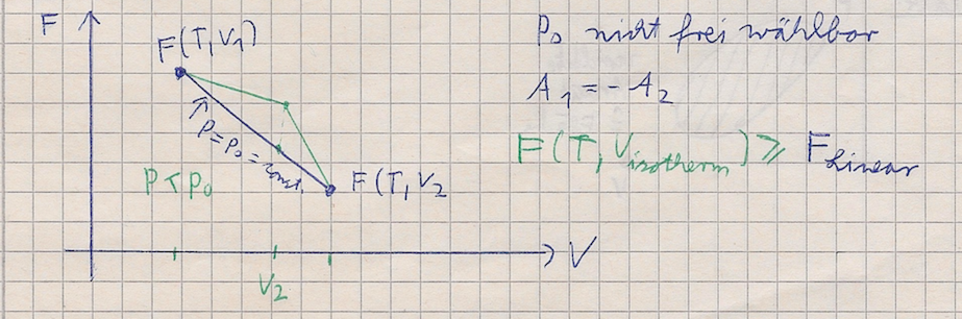
\includegraphics[width = \textwidth]{Zeichnungen/17.pdf}
  \caption{Freie Energie in Abhängigkeit vom Volumen.}
  %\label{fig:Bild}
\end{figure}











%So, Schnellkurs für Lukas :X
%\underbrace{x}_{bla} macht eine geschweifte klammer unter x, in der bla steht
%\underarrow{x}{y} macht einen Pfeil
%\pdif{x}{y}[z] macht partielle Ableitung von x nach y bei konstantem z
%\tdif{x}{x} macht totale Ableitung von x nach y
%\dif macht ein d für integrale und so
%\e macht ein gerades e
%\Tr macht Trace
%\cancel{xyz} streicht xyz durch
%\Aboxed{} macht ein kästchen drum
%Clusterfuck:
%    \cluster \\
%    \cluster[1]\\
%    \cluster[1][2]\\
%    \cluster[1][2][3] \\
%    \clustertri{1}{2}{3}\\
%    \cluster[][]